\documentclass[10pt,a4paper]{article}

% ── Packages ──────────────────────────────────────────────────────────────
\usepackage[utf8]{inputenc}
\usepackage[T1]{fontenc}
\usepackage{lmodern}
\usepackage{amsmath}
\usepackage[margin=1.2cm]{geometry}
\usepackage[hidelinks]{hyperref}
\usepackage{enumitem}
\usepackage{booktabs}
\usepackage{graphicx}
\usepackage{xcolor}
\usepackage{parskip}
\usepackage{fancyhdr}

% Formats lists tighter by default
\setlist{noitemsep,topsep=0pt,parsep=0pt,partopsep=0pt}

% ── Header / Footer ─────────────────────────────────────────────────────
\pagestyle{fancy}
\fancyhf{}
\rhead{\small EnduranceLife API --- Technical Report}
\lhead{\small David Feng}
\rfoot{\small Page \thepage}

% ── Title ────────────────────────────────────────────────────────────────
\title{%
  \textbf{EnduranceLife API} \\[0.3em]
  \large Technical Report: Design Choices, Architecture \& Reflections
}
\author{David Feng}
\date{April 2026}

\begin{document}
\maketitle
\thispagestyle{fancy}

% ══════════════════════════════════════════════════════════════════════════
\section*{Project Deliverables Links}
% ══════════════════════════════════════════════════════════════════════════
To directly satisfy the assessment requirements, all project deliverables are hyperlinked below:

\begin{itemize}[leftmargin=1.5em]
    \item \textbf{Public GitHub Repository:} \url{https://github.com/DavidFeng-8844/EnduranceLife}
    \item \textbf{API Documentation (Swagger UI):} \url{https://endurancelife.onrender.com/docs}
    \item \textbf{API Documentation (ReDoc Extracted PDF):} Available in the repo at \texttt{docs/api\_documentation.pdf}.
    \item \textbf{Presentation Slides (PDF Format):} \url{https://github.com/DavidFeng-8844/EnduranceLife/blob/main/docs/presentation.pdf}
\end{itemize}

% ══════════════════════════════════════════════════════════════════════════
\section{Introduction}
% ══════════════════════════════════════════════════════════════════════════

EnduranceLife is a RESTful Web Service API designed for managing endurance-sport training data. It ingests workout recordings from Coros GPS watches (via \texttt{.fit} files), cross-references them with daily lifestyle metrics (sleep, nutrition, fatigue) and physiological snapshots (VO2Max, resting heart rate), and exposes five analytics endpoints that produce chart-ready JSON for front-end dashboards.

The service is deployed on \href{https://endurancelife.onrender.com}{Render.com} with a managed PostgreSQL database, while retaining full local-development compatibility via SQLite.

% ══════════════════════════════════════════════════════════════════════════
\section{Technology Stack \& Justification}
% ══════════════════════════════════════════════════════════════════════════

\subsection{Programming Language: Python 3.11}

Python was chosen for three reasons:
\begin{enumerate}[leftmargin=1.5em]
  \item \textbf{Ecosystem fit.} The \texttt{fitdecode} library --- the only decoder that tolerates Coros's non-standard FIT field sizing --- is a Python package. Using Python eliminates the need for cross-language interop.
  \item \textbf{Rapid prototyping.} Dynamic typing and a concise syntax accelerated development of the four data-pipeline scripts and the analytics endpoint logic.
  \item \textbf{Data-science readiness.} Future extensions (e.g.\ ML-based race prediction, anomaly detection) can leverage Python's NumPy / scikit-learn ecosystem without rewriting the service.
\end{enumerate}

\subsection{Framework: FastAPI}

FastAPI was selected over Flask and Django REST Framework (DRF):

\begin{table}[h]
\centering
\begin{tabular}{@{}lll@{}}
\toprule
\textbf{Criterion} & \textbf{FastAPI} & \textbf{Alternatives} \\
\midrule
Auto-generated docs & Swagger + ReDoc built-in & Flask: manual; DRF: partial \\
Type validation      & Pydantic V2 (native)     & Flask: add-on; DRF: serializers \\
Async support        & First-class ASGI         & Flask: WSGI; DRF: partial \\
Performance          & Comparable to Go/Node    & Flask/DRF notably slower \\
Learning curve       & Minimal boilerplate      & DRF: steeper \\
\bottomrule
\end{tabular}
\caption{Framework comparison matrix}
\end{table}

FastAPI's automatic OpenAPI schema generation was particularly valuable: every endpoint is immediately testable via the \texttt{/docs} Swagger UI and documented via \texttt{/redoc}, satisfying the project's requirement for a self-documenting API with zero additional tooling.

\subsection{ORM: SQLAlchemy 2.0}

SQLAlchemy provides database-agnostic ORM mapping, enabling the same Python model classes to work against both SQLite (local development and testing) and PostgreSQL (production on Render). This dual-backend strategy was implemented with a single environment-variable check in \texttt{database.py}.

\subsection{Database: PostgreSQL (Production) / SQLite (Development)}

\begin{itemize}[leftmargin=1.5em]
  \item \textbf{PostgreSQL} was chosen for production because Render offers a managed free-tier instance, it is a fully relational SQL database satisfying the coursework requirement, and it supports concurrent connections from the Uvicorn worker processes.
  \item \textbf{SQLite} is used locally and in tests for zero-configuration development. The in-memory SQLite backend makes the 66-test suite execute in under 2 seconds with complete isolation.
  \item \textbf{Why not NoSQL?} The data model is inherently relational: activities reference a user (\texttt{pid}), daily metrics are keyed by \texttt{(pid, date)}, and analytics queries rely on SQL aggregations (\texttt{GROUP BY}, \texttt{SUM}, \texttt{MIN}). A document store would complicate these cross-entity joins.
\end{itemize}

\subsection{Deployment: Render.com}

Render was chosen for its GitHub-integrated CI/CD pipeline, free PostgreSQL tier, and automatic HTTPS. The deployment requires only two configuration values: installing dependencies via \texttt{pip} and running the ASGI app via \texttt{uvicorn}. A \texttt{.python-version} file pins the runtime to Python 3.11.7 to ensure pre-built wheels are available for \texttt{pydantic-core} (which requires Rust compilation on unsupported versions).

% ══════════════════════════════════════════════════════════════════════════
\section{Architecture \& Design Decisions}
% ══════════════════════════════════════════════════════════════════════════

\subsection{Project Structure}

The codebase follows a \textbf{domain-driven router pattern}. The entry point (`main.py`) integrates routers (`auth.py`, `activity.py`, `daily\_metric.py`, `physiology.py`, `analytics.py`), database configurations, ORM models, and Pydantic validation schemas. Each router owns a single URL prefix and tag, keeping concerns isolated and enabling independent testing.

\subsection{Data Pipeline Architecture \& API Endpoints}

The core data ingestion is handled through endpoints in the API and four standalone ETL scripts in \texttt{scripts/}:

\begin{enumerate}[leftmargin=1.5em]
  \item \textbf{File Uploads \& FIT Parsing (\texttt{/activities/upload}):} Rather than relying entirely on manual JSON entry, the API accepts binary \texttt{.fit} files (the standard used by Garmin, Coros, Wahoo) via \texttt{multipart/form-data}. The upload endpoint delegates parsing to the \texttt{fitdecode} library. It iterates through the file frames to extract bounding timestamps (start, end), total distance, elevation ascent/descent, and computes metrics like average pace or heart rate dynamically from the data stream. Finally, these parsed metrics are automatically mapped to the SQLAlchemy \texttt{Activity} ORM and inserted into the PostgreSQL database.
  \item \textbf{RESTful Pagination \& Filtering (\texttt{/activities/} \& \texttt{/daily-metrics/}):} The list endpoints utilize query parameters (\texttt{skip}, \texttt{limit}, \texttt{date\_from}, \texttt{date\_to}, \texttt{pid}) to dynamically construct SQLAlchemy `.filter()` clauses. This pushes the filtering down to the database engine level (e.g., executing \texttt{WHERE user\_id = 1 AND start\_time >= '2025-01-01'}), preventing memory bloat by returning only the paginated slice of records requested.
  \item \textbf{Composite-Key Updates (\texttt{PUT /daily-metrics/by-date}):} The Daily Metrics router implements an upsert/update strategy based on a composite business key (\texttt{pid} + \texttt{date}). This allows smart integrations (or frontend clients) to send a payload for ``today's stats'' without needing to perform a prior \texttt{GET} request to look up the database's internal row ID, significantly reducing network overhead.
  \item \textbf{Data Enrichment Pipeline:} Supplemental standalone scripts execute batched background operations. \textbf{import\_fit.py} handles directory-wide ingestion. \textbf{enrich\_weather.py} calls the external Open-Meteo API using latitude/longitude extracted from activities to backfill missing environmental data. \textbf{seed\_daily\_metrics.py} \& \textbf{seed\_physiology.py} generate correlated simulated lifestyle data and physiological progressions (using sine-wave trending and randomized fatigue noise) to provide realistic sample testing datasets.
\end{enumerate}

All scripts use \textbf{batch commits} (configurable, default 30--50 records per flush) and \textbf{in-memory duplicate detection} (pre-loading existing keys into a \texttt{set()}) to minimize network round-trips when operating against a remote PostgreSQL instance.

\subsection{Analytics Engine}

The five analytics endpoints (\texttt{/analytics/*}) are designed as \textbf{complex SQL aggregations} routed directly into Pydantic response models. By offloading computation to the database layer (PostgreSQL), the API minimizes memory usage. Key implementations include:

\begin{itemize}[leftmargin=1.5em]
  \item \textbf{Race Predictor / Physiology Trends:} Uses the Daniels VO2-velocity quadratic formula ($\mathrm{VO2} = -4.60 + 0.182258v + 0.000104v^2$) iteratively solved or derived. The algorithm is mapped in Python to convert the user's latest recorded \texttt{vo2\_max} logarithmically into sustainable pace forecasts for 5K, 10K, and Half Marathons. It uses calibrated sustainability factors (e.g., humans cannot indefinitely hold VO2Max; 5K pace operates at ~95\% VO2Max, HM at ~85\%).
  \item \textbf{Performance Records (PR Filtering Engine):} Tracks fixed-distance best times by grouping and ranking activities. Crucially, the logic involves rigorous \textbf{anomaly filtering}. GPS errors frequently record impossible pacings. The logic excludes data outside physiologically plausible bounds ($<$ 2:30/km or $>$ 10:00/km for runs; $<$ 8 km/h or $>$ 70 km/h for rides).
  \item \textbf{Environment Insights (Temperature Bucketing):} Utilizing SQLAlchemy's Conditional Expressions (\texttt{case} statements), weather data is bucketed dynamically. The query groups activities into three thermal constraints: Cold ($<10^\circ$C), Moderate ($10-22^\circ$C), and Hot ($>22^\circ$C). Averages for heart rate and speed are then computed \textit{per bucket} via \texttt{func.avg()}, mathematically illustrating the exact cardiovascular drift caused by extreme heat.
  \item \textbf{Lifestyle Impact (Cross-Table Joins):} Correlates the \texttt{daily\_metrics} table (subjective fatigue, sleep hours) with the \texttt{activities} table (objective pace, heart rate). Utilizing SQL \texttt{JOIN} clauses on \texttt{date(start\_time) == date}, the endpoint categorizes performance against sleep states (e.g., comparing days with $>$7h sleep vs $<$6h sleep) to expose behavioral trends.
\end{itemize}

\subsection{Dual-Database Strategy}

A single three-line conditional in \texttt{database.py} enables seamless switching:

The application reads the \texttt{DATABASE\_URL} environment variable. If present (like in the Render environment), it configures a PostgreSQL connection. If absent (local environment), it defaults to a local SQLite database file, enabling seamless testing and deployment without code changes.

This pattern requires zero code changes between local development, CI testing (in-memory SQLite), and production deployment (Render PostgreSQL).

\subsection{Authentication}

The API implements JWT-based authentication with four endpoints:

\begin{itemize}[leftmargin=1.5em]
  \item \texttt{POST /auth/register} --- Create a new user (bcrypt-hashed password storage).
  \item \texttt{POST /auth/login} --- Verify credentials and return a signed JWT (30~min expiry, configurable via \texttt{TOKEN\_EXPIRE\_MINUTES}).
  \item \texttt{POST /auth/logout} --- Invalidate the token by blacklisting its unique \texttt{jti} (JWT ID) claim.
  \item \texttt{GET /auth/me} --- Return the authenticated user's profile.
\end{itemize}

\textbf{Key design choices:}
\begin{itemize}[leftmargin=1.5em]
  \item \textbf{Global Data Isolation (IDOR Prevention):} To prevent Insecure Direct Object Reference vulnerabilities, the \texttt{pid} field is stripped from all client payloads and query parameters. Instead, the \texttt{get\_current\_user} FastAPI dependency uses token extraction to tightly scope all SQL CRUD operations and Analytics aggregations exclusively to the logged-in user's ID (\texttt{current\_user.id}).
  \item Each JWT contains a UUID-based \texttt{jti} claim, ensuring that tokens issued in the same second are distinguishable and can be blacklisted independently.
  \item The \texttt{get\_current\_user} dependency is injected into all 23 protected routes to enforce authentication synchronously.
  \item The blacklist is in-memory (a Python \texttt{set}); in production, this would be replaced with Redis or a database table for persistence across restarts.
  \item \textbf{Pre-seeded Demo User.} To facilitate evaluating the populated dashboard analytics data smoothly, an application startup hook automatically seeds a default user (\texttt{username: demo}, \texttt{password: endurance2026}) as user \texttt{id=1} if the database is empty. All generated mock data routes to this \texttt{pid=1}. \textit{(Testing Note: Evaluators should use the global ``Authorize'' button at the top of the Swagger UI rather than executing the \texttt{/auth/login} block manually. The global button natively extracts the stateless JWT from the HTTP 200 response and seamlessly injects it into all future requests, accurately simulating a frontend client state.)}
\end{itemize}

% ══════════════════════════════════════════════════════════════════════════
\section{Testing Approach}
% ══════════════════════════════════════════════════════════════════════════

The project maintains an \textbf{80-test suite} using \texttt{pytest}, covering all CRUD operations, analytics routes, and authentication layers. Every test session spins up a fresh \texttt{sqlite:///:memory:} database via a pytest fixture, ensuring complete isolation and sub-2-second execution. Tests rigorously verify edge causes, such as 409 conflicts, 422 validations, anomaly filtering thresholds, and data isolation logic. Layered fixtures in \texttt{conftest.py} efficiently seed the database state without boilerplate.

% ══════════════════════════════════════════════════════════════════════════
\section{Challenges \& Lessons Learned}
% ══════════════════════════════════════════════════════════════════════════

Several key lessons were learned during development:
1) \textbf{Data Parsing:} Native Coros watches produce non-standard FIT byte packing, requiring the use of \texttt{fitdecode} over \texttt{fitparse}.
2) \textbf{Route Ordering:} FastAPI evaluates routes sequentially; parameterized paths must strictly follow explicit literal endpoints to prevent shadowing.
3) \textbf{Database Tuning:} Initial imports to Render's cloud PostgreSQL took 10+ minutes due to high network round-trips. Refactoring to batch inserts dropped this to under 3 minutes, highlighting the difference between local SQLite and remote deployments.
4) \textbf{Environment Hurdles:} We explicitly pinned Python 3.11 \texttt{.python-version} to fix Rust compilation errors during deployment, and rerouted CDN assets to \texttt{unpkg.com} to bypass regional blocks on Swagger dependencies.

% ══════════════════════════════════════════════════════════════════════════
\section{Limitations \& Future Work}
% ══════════════════════════════════════════════════════════════════════════

While the API architecture successfully implements Zero-Trust data isolation and robust analytics, a few limitations persist. Schema migrations are currently raw metadata creations rather than versioned \texttt{Alembic} migrations. Furthermore, the token blacklist is in-memory and volatile upon restarts; production deployment would warrant an external \texttt{Redis} cache. 

Future extensions could transform this RESTful structure into a real-time SPA dashboard via WebSockets and React/Vue.js (using ECharts). Additional features might include OAuth-sync directly with hardware APIs (Garmin Connect) and upgrading the mathematical Daniel’s VO2 Formula predictions with localized Machine Learning regression models trained exclusively on user historical outputs.



% ══════════════════════════════════════════════════════════════════════════
\section{Cloud Deployment \& Evidence}
% ══════════════════════════════════════════════════════════════════════════

The API is fully deployed into a production cloud environment on Render, utilizing a managed PostgreSQL database. To facilitate continuous operation and frictionless evaluation, the deployment integrates an idempotent automatic seeding script (\texttt{scripts.seed\_db}) in the web service Start Command. This ensures the PostgreSQL database always retains a functional, analytics-ready ``demo'' user dashboard upon instantiation.

The successfully deployed endpoints can be explored live via the Swagger UI interface: \url{https://endurancelife.onrender.com/docs}.

\begin{figure}[ht]
    \centering
    \begin{minipage}{0.48\textwidth}
        \centering
        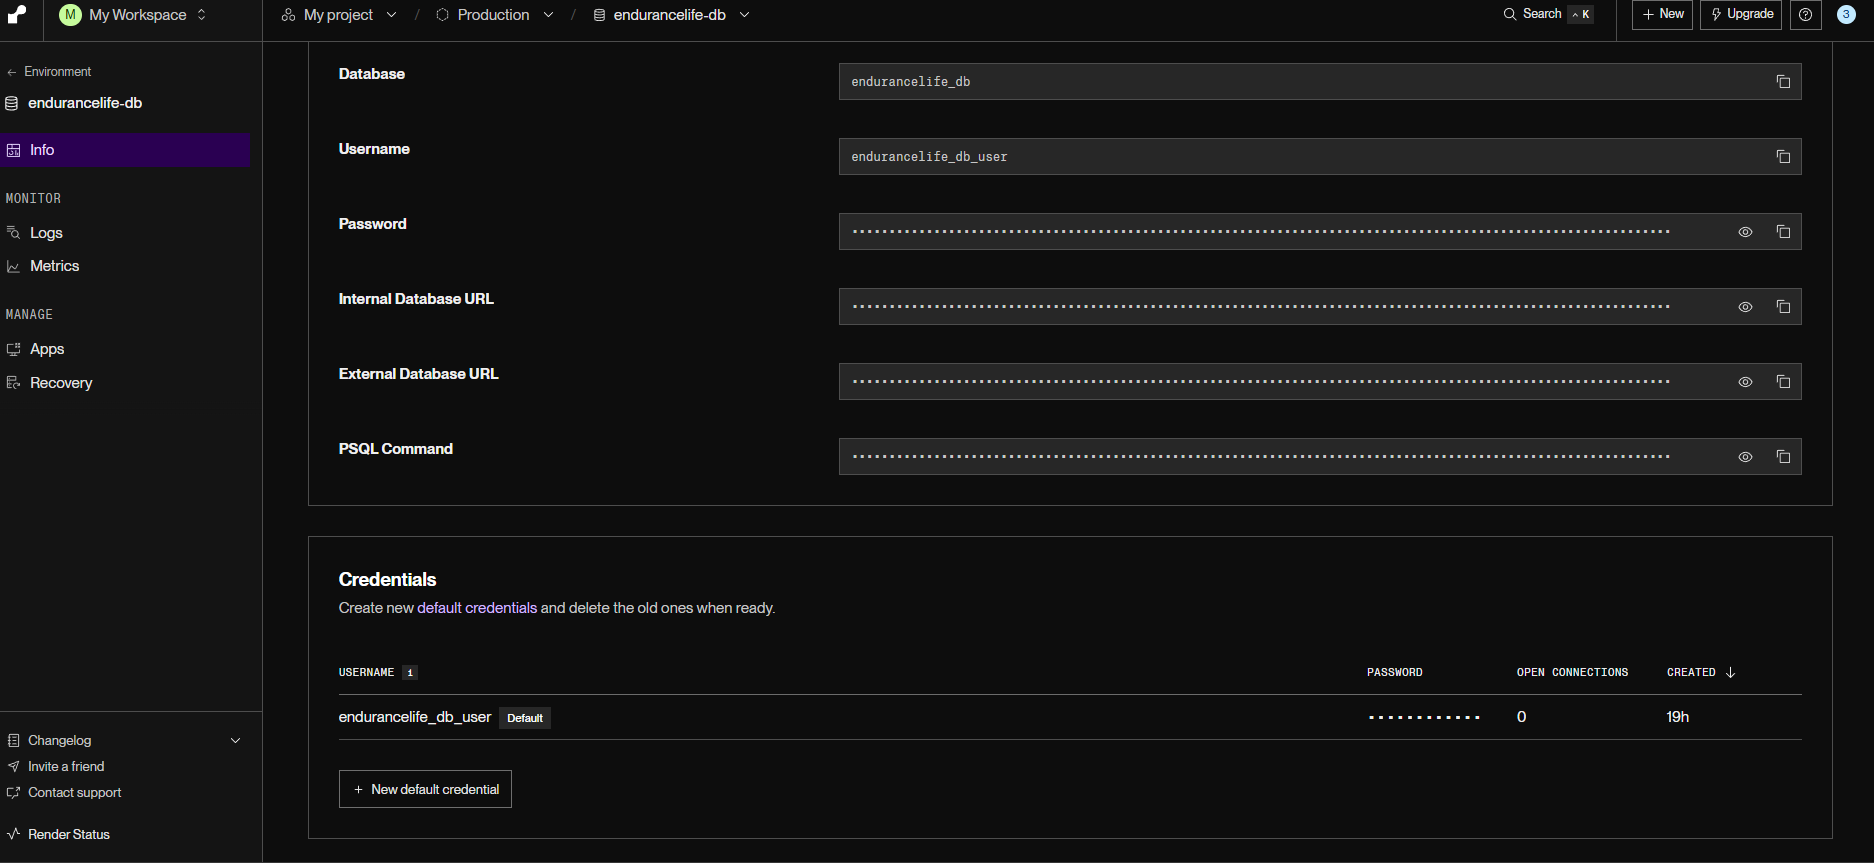
\includegraphics[width=0.9\linewidth]{db_screenshot.png}
        \caption{PostgreSQL Instance}
    \end{minipage}\hfill
    \begin{minipage}{0.48\textwidth}
        \centering
        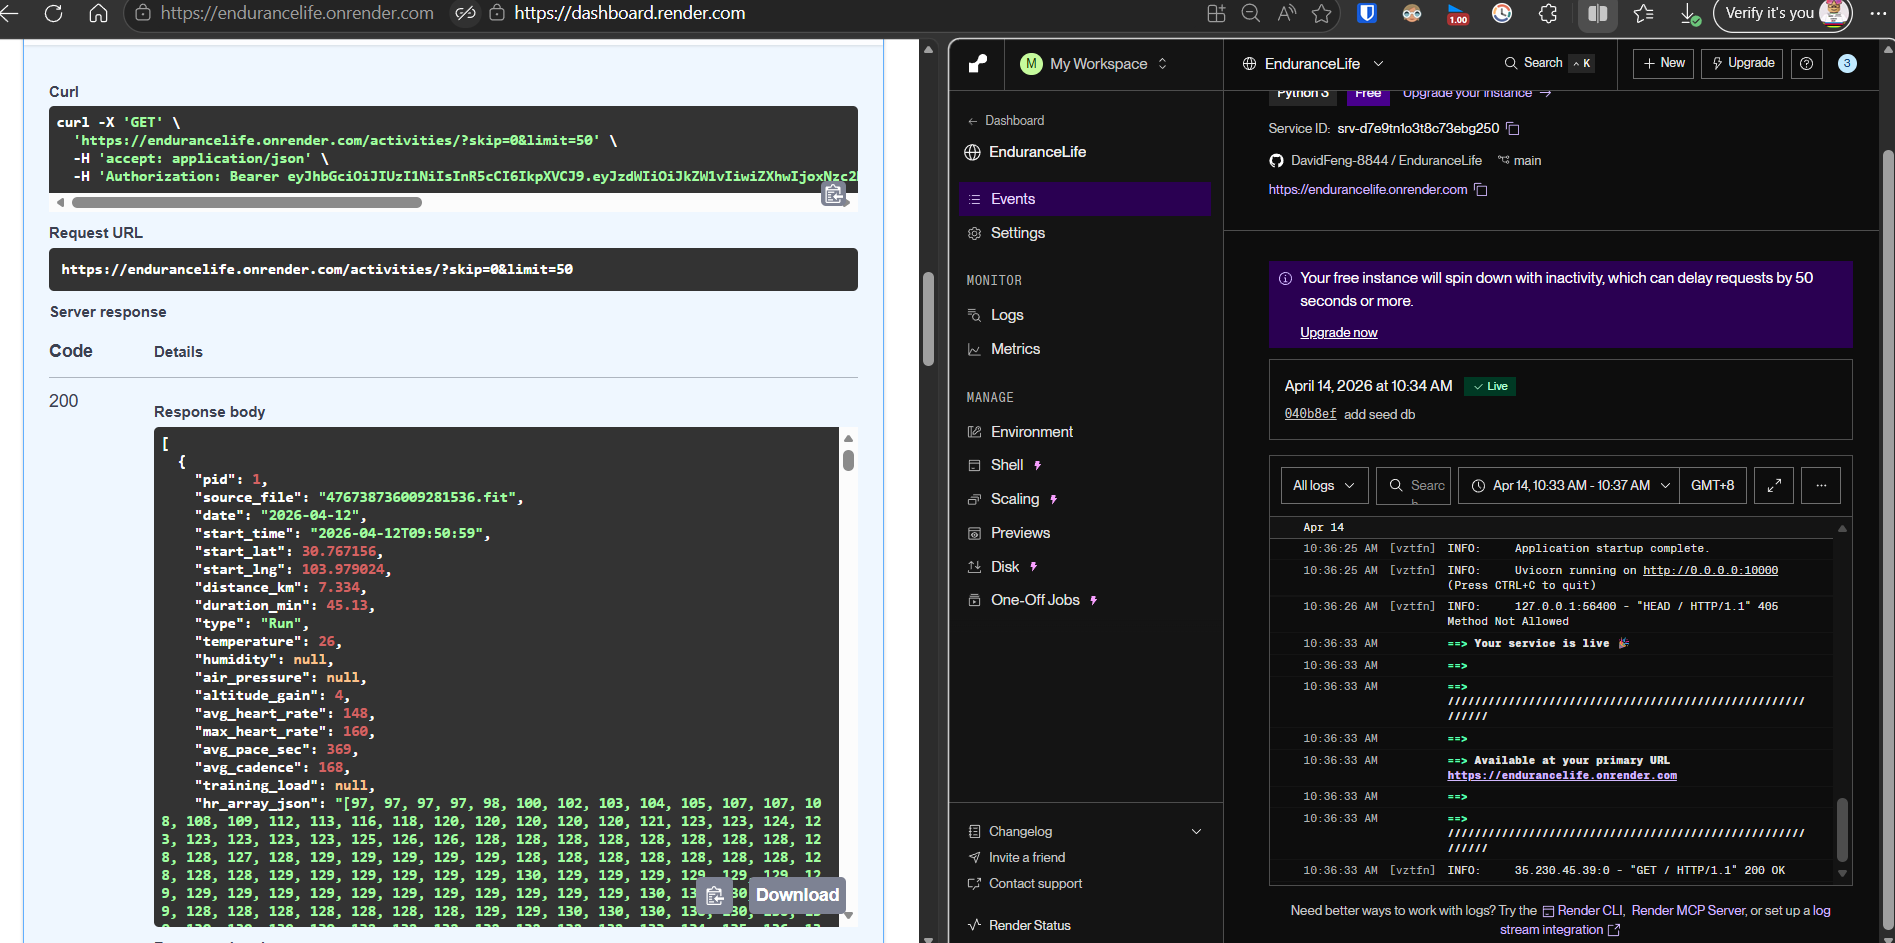
\includegraphics[width=0.9\linewidth]{swagger-ui_split-screen-get-activity_render-control-center-log_screenshot.png}
        \caption{Server Logs \& Swagger}
    \end{minipage}
\end{figure}

% ══════════════════════════════════════════════════════════════════════════
\section{Conclusion}
% ══════════════════════════════════════════════════════════════════════════

EnduranceLife demonstrates a complete RESTful API lifecycle: domain modelling, CRUD operations, file upload handling, external API integration, analytics computation, comprehensive testing, and cloud deployment. The technology choices --- Python, FastAPI, SQLAlchemy, PostgreSQL --- form a cohesive stack that balances development speed with production readiness. The dual-database strategy and batch-optimized data pipelines address the practical challenges of deploying a data-intensive application to a free-tier cloud platform.

% ══════════════════════════════════════════════════════════════════════════
\section{References}
% ══════════════════════════════════════════════════════════════════════════

\begin{itemize}[leftmargin=1.5em]
    \item \textbf{Core Frameworks:} FastAPI (\url{https://fastapi.tiangolo.com/}), Pydantic V2, and SQLAlchemy ORM.
    \item \textbf{Libraries utilized:} \texttt{fitdecode} for binary parsing of smartwatch workouts; \texttt{passlib} and \texttt{python-jose} for JWT generation and bcrypt password hashing.
    \item \textbf{External APIs \& Datasets:}
    \begin{itemize}[label=$\circ$]
        \item Open-Meteo Historical Weather API (\url{https://open-meteo.com/}) utilized in \texttt{enrich\_weather.py} to backfill environmental context.
        \item Native Coros smartwatch \texttt{.fit} export files (personal dataset) utilized as the seed data payload.
    \end{itemize}
    \item \textbf{Theory \& Tutorials:}
    \begin{itemize}[label=$\circ$]
        \item \textit{Daniels' Running Formula} by Jack Daniels (mathematical basis utilized in \texttt{analytics.py} to compute sustainable continuous fractional VO2 velocity predicts).
        \item Render.com deployment specifications and cloud PostgreSQL connection tutorials (\url{https://render.com/docs}).
    \end{itemize}
\end{itemize}

\appendix
% ══════════════════════════════════════════════════════════════════════════
\section{Generative AI Usage, Disclosure \& Analysis}
% ══════════════════════════════════════════════════════════════════════════

\subsection{Declaration of Use}

Generative AI tools were used during the development of this project. Specifically, \textbf{Google Gemini (via Antigravity IDE)} was used as a pair-programming assistant throughout the development process.

\subsection{How AI Was Used}

\begin{enumerate}[leftmargin=1.5em]
  \item \textbf{Code generation.} AI generated initial implementations of CRUD routers, Pydantic schemas, and test fixtures. Every generated block was reviewed, tested, and frequently modified to fit the project's conventions.
  \item \textbf{Algorithm calibration.} The Daniels VO2-velocity formula implementation was iteratively refined with AI assistance, cross-referencing the mathematical model against my real-world 5K and half-marathon performance data to calibrate sustainability factors.
  \item \textbf{Debugging.} AI identified the FastAPI route-ordering conflict and the Render Python version incompatibility, both of which would have required significant manual investigation.
  \item \textbf{Performance optimization.} The batch-commit refactoring of all four data-pipeline scripts was developed collaboratively with AI, discussing trade-offs between memory usage and network round-trips.
  \item \textbf{Documentation.} This report's structure was drafted with AI assistance, though all technical content reflects my actual design decisions and real development experience.
\end{enumerate}

\subsection{Critical Reflection}

AI accelerated development significantly --- the 80-test suite and five analytics endpoints were built in a fraction of the time manual development would have required. However, AI assistance also introduced risks:

\begin{itemize}[leftmargin=1.5em]
  \item \textbf{Over-reliance on suggestions.} The initial race prediction formula generated by AI was mathematically incorrect (a simplistic linear model). It required manual verification against published sports-science research (Daniels' Running Formula) and calibration against real data to produce accurate predictions.
  \item \textbf{Platform-specific blindspots.} AI initially used Unicode box-drawing characters in print statements that crashed on Windows' CP1252 terminal encoding. Real-world testing caught this.
  \item \textbf{Shallow understanding.} AI suggested the \texttt{StandaloneLayout} preset for Swagger UI without loading the required standalone preset JavaScript file, causing a runtime error. This was caught by manual testing on the deployed instance.
\end{itemize}

\textbf{Conclusion:} AI is a powerful productivity multiplier, but it does not replace domain expertise, manual testing, or critical review. Every AI-generated artifact was validated before integration, and several were corrected or discarded. The final codebase reflects a collaborative human-AI development process where human judgement remained the quality gate.

\subsection{Conversation Logs}
The complete conversation logs covering all interactions, prompts, iterations, and analyses with the Generative AI are included alongside this submission as required by the grading criteria (available securely in the delivery package repository / zip file).

\end{document}
